
\documentclass{MScthesisITEM}

% this package is just to generate text for demo-purposes
\usepackage{blindtext}
\usepackage{hyperref}


\title{Runtime Systems for State Machines \newlinetitle in Lua} % The title of your assignement; NB use \newlinetitle to start a newline
\author{\O yvin Richardsen} % Your firstname and lastname
\professor{Frank Alexander Kraemer; NTNU Department of Telematics, Bitreactive} % Affiliation = ITEM for instance
\supervisor{Frank Alexander Kraemer; NTNU Department of Telematics, Bitreactive}

%% Uncomment the following in case you want subfigures; note that there will be a warning for the caption package
% \let\subcaption\undefined
% \let\subfloat\undefined
% \usepackage[bf]{caption}
% \usepackage{subcaption}

\DeclareGraphicsExtensions{.pdf,.jpg}
\graphicspath{{./figs/}}

\loadglsentries{glossary}
\makeglossaries

\begin{document}
\selectlanguage{english}
\pagenumbering{roman}
\pagestyle{plain}

%% Only for the project
\titleITEM

%% Only for the master's thesis; for the project report the description is taken from It's Learning and added by the department
% \selectlanguage{english} % Change to 'norsk' if you are writing in Norwegian
% \begin{titlingpage}

\noindent
\begin{tabular}{@{}p{4cm}l}
\textbf{Title:} 	& \thetitle \\
\textbf{Student:}	& \theauthor \\
\end{tabular}

\vspace{4ex}
\noindent\textbf{Problem description:}
\vspace{2ex}

\noindent \Blindtext[2][1]
\vspace{6ex}

\noindent
\begin{tabular}{@{}p{4cm}l}
\textbf{Responsible professor:} 	& \theprofessor \\
\textbf{Supervisor:}			& \thesupervisor \\
\end{tabular}

\end{titlingpage}
% \cleardoublepage

%% There must be an abstract in English, even though the main text is in Norwegian
\selectlanguage{english}
\pagestyle{empty}
\begin{abstract}
%\noindent \Blindtext[5][1]
\end{abstract}
\cleardoublepage

%% Only for the master's thesis; if the main text is in English and you can write Norwegian, there must be an abstract in Norwegian as well.A
% \selectlanguage{norsk}
% \pagestyle{empty}
\renewcommand{\abstractname}{Sammendrag}
\begin{abstract}
\noindent Sikkerheten til nesten all offentlig nøkkel-kryptografi er basert på et vanskelig beregnbarhetsproblem. Mest velkjent er problemene med å faktorisere heltall i sine primtallsfaktorer, og å beregne diskrete logaritmer i endelige sykliske grupper. I de to siste tiårene, har det imidlertid dukket opp en rekke andre offentlig nøkkel-systemer, som baserer sin sikkerhet på helt andre type problemer. Et lovende forslag, er å basere sikkerheten på vanskeligheten av å løse store likningsett av flervariable polynomlikninger. En stor utfordring ved å designe slike offentlig nøkkel-systemer, er å integrere en effektiv ``falluke'' (trapdoor) inn i likningssettet. En ny tilnærming til dette problemet ble nylig foreslått av Gligoroski m.f., hvor de benytter konseptet om kvasigruppe-strengtransformasjoner (quasigroup string transformations). I denne masteroppgaven beskriver vi en metodikk for å identifisere sterke og svake nøkler i det nylig foreslåtte multivariable offentlig nøkkel-signatursystemet MQQ-SIG, som er basert på denne idéen.

Vi har gjennomført et stort antall eksperimenter, basert på Gröbner basis angrep, for å klassifisere de ulike parametrene som bestemmer nøklene i MQQ-SIG. Våre funn viser at det er store forskjeller i viktigheten av disse parametrene. Metodikken består i en klassifisering av de forskjellige parametrene i systemet, i tillegg til en innføring av konkrete kriterier for hvilke nøkler som bør velges. Videre, har vi identifisert et unødvendig krav i den originale spesifikasjonen, som krevde at kvasigruppene måtte oppfylle et bestemt kriterie. Ved å fjerne denne betingelsen, kan nøkkel-genererings-algoritmen potensielt øke ytelsen med en stor faktor. Basert på alt dette, foreslår vi en ny og forbedret nøkkel-genereringsalgoritme for MQQ-SIG, som vil generere sterkere nøkler og være mer effektiv enn den originale nøkkel-genereringsalgoritmen.  
\end{abstract}
% \cleardoublepage

\selectlanguage{english}% Change to 'norsk' if you are writing in Norwegian

\renewcommand{\abstractname}{Preface}
\begin{abstract}
\noindent
This paper is the report written as part of the specialization project course taken in the 9th semester (fall 2013) of my 5-year MSc in Communication Technology at the \gls{ntnu}, awarding 15 ECTS credits. It is focused around the experimental process of determining whether or not the Lua programming language is suited for developing state machine systems on embedded, memory-constrained devices.

\noindent
This process has given me more insight in various topics related to both programming language semantics and working with software on embedded devices, which to me is quite interesting. Hopefully, the report will be interesting and offer some new insights also to the reader.

\noindent
I would like to thank my supervisor, Frank Alexander Kraemer for useful advice during my work, especially in the early phases. I would also like to thank my good friend Sandor Zeestraten for taking the time to read through and comment on the report. \\
\\
\\
Øyvin Richardsen
\end{abstract}
\cleardoublepage

% similarly you may add a separate acknowledgments page

\tableofcontents*
\cleardoublepage

%% include if relevant
\listoffigures
\cleardoublepage

%% include if relevant
\listoftables
\cleardoublepage

%% include if relevant
\listofalgorithms
\addcontentsline{toc}{chapter}{List of Algorithms}
\cleardoublepage

%% include if relevant
\printglossary[title=List of Symbols, style=long]
\cleardoublepage
\glsaddall[]

%% include if relevant
\printglossary[title=List of Acronyms,type=\acronymtype] % prints just the list of acronyms
\cleardoublepage

\pagenumbering{arabic}
\pagestyle{ruled}
%\chapter{Introduction}
\label{chp:intro}

\chapter{Background}
\label{chp:background}

\section{The Lua programming language}
\label{sec:lua_language}

The Lua programming language is a dynamic, multi-paradigm scripting language developed at the Pontifical Catholic University of Rio de Janeiro. Some key properties of Lua:

\begin{itemize}
	\item TODO: rewrite this
	\item Dynamically typed
	\item Interpreted scripting language
	\item Simple but powerful syntax, meta-mechanisms
	\item Simple and well-documented API for integration with other languages
	\item Collaborative multithreading
	\item Lua VM is written in "clean C"
	\item Compiled to bytecode, to be run in the Lua VM
	\item Register-based VM
	\item Incremental mark-and-sweep garbage collector
	\item Distributed under the very liberal MIT license \cite{website:lua_license}
\end{itemize}

While Lua is designed as an extension scripting language mainly for C, it is still possible to execute standalone Lua programs through the Lua interpreter \cite[ch. 7]{book:lua_reference_manual}.

Lua is the most popular interpreted scripting language for games \cite{website:the_engine_survey}.

\section{State machine -based systems}


\section{Embedded systems and M2M}
\chapter{Previous and related work}
\label{ch:related_work}
This chapter outlines work done by other people related to my problem description. It has two main sections: the first part describes existing frameworks for creating state machine -based systems, and the second part outlines some previous attempts at working with Lua in embedded systems. I have not been able to find any previous work combining the two topics, so I will assume it is a fairly untouched field.

\section{Existing frameworks for state machine applications}
\label{sec:existing_frameworks_state_machine}
State machine -based systems is a well-established concept in the world of software, and several frameworks already exist for developing applications based on this concept. These frameworks vary in implementation language, design method and portability, and some of their main properties will be outlined in this section. These frameworks will be used for comparison when evaluating Lua/eLua for state machine -based systems.

\subsection{Reactive Blocks}
\label{sec:reactive_blocks}
Reactive Blocks (\url{http://www.bitreactive.com})is a Java-based framework for developing state machine applications. It offers integration with the Eclipse IDE, and is essentially a code/application generator with a graphical interface, tailored for event-driven and concurrent systems. Application design is done by creating, connecting and combining various “building blocks”. These building blocks consist of three parts:
\begin{itemize}
	\item Activity diagram \ref{state_machine_systems}: describes the internal behavior and logic of the block.
	\item External state machine: serves as an interface towards other blocks and the enclosing application. Defines which input signals are allowed in a given state, transitions associated with an input signal and a state, and any output signals resulting from the transition.
	\item Java methods that handle any operations performed as part of a transition.
\end{itemize}

An example of a building block in Reactive Blocks is displayed in figure \ref{figure:reactive_blocks}.

\begin{figure}[h]
	\centering
	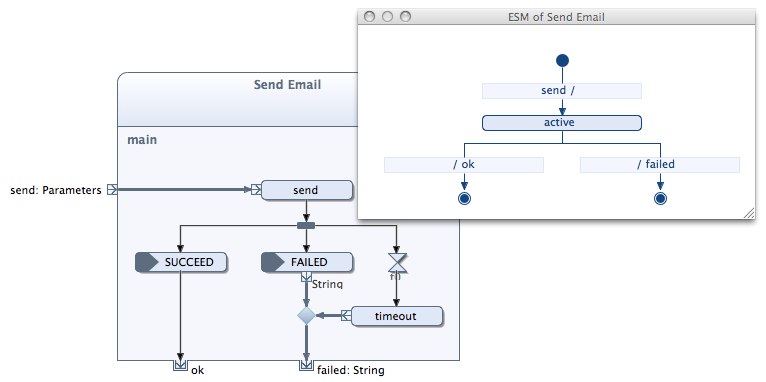
\includegraphics[scale=0.5]{img/reactive_blocks.png}
	\caption[A building block in Reactive Blocks]{An example of a building block in Reactive Blocks, displaying the activity diagram (to the left) and the external state machine (to the right). Image source: \url{http://reference.bitreactive.com/doc/building_blocks} \label{figure:reactive_blocks} }
\end{figure}

The Reactive Blocks SDK has various advantages for development of state machine -based applications:
\begin{itemize}
	\item It comes with a built-in verification tool that helps the user discover and handle logical mistakes and design flaws in the application. The framework also integrates with JUnit, for testing separate components and operations.
	\item Instead of a large and complex code base, the application consists of a hierarchy of connected building blocks, with functionality and logic defined at the design level. This generally makes projects easier to organize, maintain and extend.
	\item With the built-in runtime support system and implementation at the design level, concepts like forking, waiting and synchronization are simple, making creation of concurrent systems almost a triviality.
	\item Java has a huge base of libraries that may be combined with Reactive Blocks to provide functionality and application development on higher levels.
\end{itemize}

However, one fundamental disadvantage is that any applications created with Reactive Blocks require a Java virtual machine. This creates an obstacle when working on embedded systems, because the Java SE Embedded VM currently only supports the \textit{most powerful} embedded systems \cite{website:java_embedded_vm}. Memory requirements range from 130KB RAM/350KB ROM (minimal configuration) to several MB for both RAM and ROM (full configuration), which is more than what you can expect to find in a typical light

\subsection{RKH}
\label{sec:rkh_state_machine}
RKH (\url{http://rkh-reactivesys.sourceforge.net}) is a C-based development tool for implementing state machine -based systems. It is specifically designed to work on embedded systems, and consists of various platform-independent modules. The software provides a cooperative scheduler, timer and event managers, as well as a graphical interface to help designing state machines based on UML state tables. Like Reactive Blocks, RKH generates and compiles code that can be run directly. An example of a transition table statement in RKH is displayed in figure \ref{figure:rkh_transition}.

\begin{figure}[h]
	\centering
	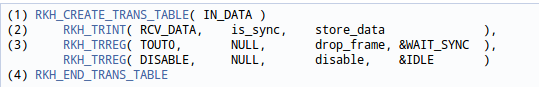
\includegraphics[scale=0.7]{img/rkh_transition_table.png}
	\caption[A transition table statement in RKH]{An example of a transition table statement in RKH, written in C code. Each line in the statement defines a transition with input signal, guard function, action function and target state. Image source: \url{http://rkh-reactivesys.sourceforge.net/qref.html} \label{figure:rkh_transition} }
\end{figure}

RKH has some particularly strong advantages when developing state machine -based applications on embedded systems:
\begin{itemize}
\item RKH is fairly platform-independent, and already built to support many platforms and processors (linux, RTOS, mbed etc…). Additionally, the modules are customizable and the project is open source, meaning it can be adapted also to custom platforms.
\item The system has a very small memory footprint, making it usable also for minimal embedded systems.
\item Application design with state tables and diagrams is simple and maintainable.
\end{itemize}

However, for the less experienced programmer, RKH also provides some challenges:
\begin{itemize}
	\item While parts of the RKH interface can be intuitively understood, other parts (like declaring actions) require at least basic knowledge of C programming. Programming in C is considered complex and difficult compared to “higher level”-languages like Java, Python or Lua.
	\item Customization and adaptation of the software platform requires knowledge of and skills in C programming.
	\item External libraries implementing functionality are fairly limited in C, and must in some cases be adapted to the relevant platform anyway. This means C programming and extra work is required for anything but standard state machine functionality.
\end{itemize}

\subsection{Quantum Leaps}
\label{sec:quantum_leaps}
Quantum Leaps (\url{http://www.state-machine.com}) offers a product for developing state machine -based applications in two parts: an active object framework, Quantum Platform (QP), and a graphical modeling tool, QP Modeler (QM).

QP is open-source, portable, C/C++ based, and built on a non-blocking, run-to-completion kernel. QP-applications consist of strictly encapsulated and asynchronously communicating active objects similar to the building blocks of Reactive Blocks described in Section \ref{sec:reactive_blocks}. The behavior of an active object is specified by an UML statechart, which can be modeled in QM. QM is a fully graphical modeling environment which generates C or C++ code according to the UML statecharts to be used with the QP framework. An example of a statechart modeled in QM is displayed in figure \ref{figure:qm_statechart}.

Some of the advantages with QP/QM are:
\begin{itemize}
	\item Memory requirements for QP are very low, and range from 2KB ROM/100B RAM (QP-nano) to 8KB ROM/1KB RAM (QP/C and QP/C++).
	\item QP is ported to a large number of platforms and processors, including ARM and AVR32 processors, Android, FreeRTOS and Arduino.
	\item QP provides automatic rule checking of the generated code.
	\item QM offers application development and implementation at the design level.
\end{itemize}

\begin{figure}[h]
	\centering
	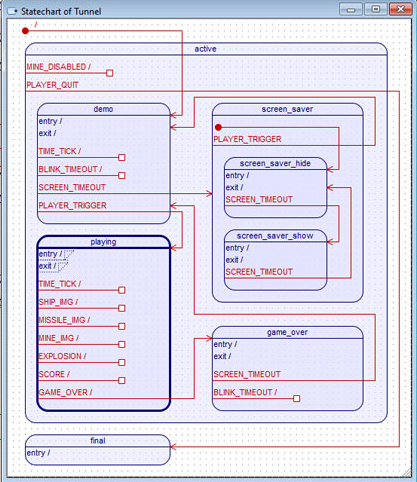
\includegraphics[scale=0.6]{img/qm_statechart.png}
	\caption[An UML statechart in QM]{A QP active object modeled as a hierarchical UML statechart in QM. Each statechart lists possible input signals and the following output signals or actions. Image source: \url{http://www.state-machine.com/qm/index.php} \label{figure:qm_statechart} }
\end{figure}

The major disadvantage with QP/QM is that it is implemented in C/C++, which means implementation of application-specific transaction operations require knowledge of C/C++ programming. However, while these are considered to be more “advanced” languages than for example Python, the level of knowledge required in this context may not be all that high (these operations can be quite simple).

\subsection{IntelliWizard}
\label{sec:intelliwizard}
\url{http://www.codeproject.com/Articles/10801/Design-State-Machine-Engine-for-embedded-system-de}
TODO

\section{Lua on embedded systems}
\label{sec:lua_on_embedded}
While Lua is primarily used as an extension and scripting language for applications written in other programming languages, it is also sometimes used to create standalone applications. Because of Lua’s small memory footprint and configurable C source code, some effort has also been made to port the Lua interpreter to various embedded systems, both with and without the need for an underlying operating system. Some of these efforts will be outlined in this section.

\subsection{LEGO Mindstorms}
\label{sec:lego_mindstorms}
In chapter 26 of “Lua programming gems” \cite{chapter:porting_lua_microcontroller}, Ralph Hempel describes his efforts in porting the Lua interpreter to a platform with severe memory constraints. His choice of platform was a LEGO MINDSTORMS NXT system with an ARM7-based microcontroller, 256KB ROM and 64K RAM. Hempel, being an experienced embedded systems programmer, used his own custom toolchain for compilation and linking. The first thing he noted in the process, was that all of the changes needed to port the basic Lua code to the ARM7 microcontroller were limited to a single file, and the Lua developers had actually created a specific space for such changes. One thing requiring quite a bit of extra work, was building a run-time library (RTL) to support Lua on the microcontroller (standard Lua uses libraries from the operating system). Hempel chose to build his own, but pointed out that a RTL is usually available from the manufacturer of the system. To reduce complexity of these libraries and make it all work within the limited resources of the platform, Hempel made some changes to the capabilities of the Lua garbage collector, the I/O system, as well as the number system used (standard Lua is based only on floating-point math \ref{sec:lua_basics}). His final conclusion was that while it is possible to port Lua to a microcontroller like the one he used, it requires a lot more work and consideration than simply adapting it to a different operating system.

\subsection{Einsatz von Lua in Embedded Systems}
\label{sec:einsatz_von_lua_embedded}
In their book “Einsatz von Lua in Embedded Systems” \cite{book:einsatz_von_lua_embedded} (translated: “Use of Lua in Embedded Systems”), Claus Kühnel and Daniel Zwirner explore the possibility of using Lua on various embedded platforms. Because of my limited understanding of German I have not read the entire book, but I have looked into parts of their work. Their arguments for using Lua on an embedded system include the speed/performance of the Lua interpreter, a low memory footprint (while still providing a full garbage collector), and easy interfacing with C code. Their experiments include using the Lua interpreter with libraries that control common embedded systems peripherals, as well as running Lua on actual embedded systems with limited resources, like mbed (\url{http://mbed.org/}). They also look into eLua, which is described in Section \ref{sec:elua}.

\subsection{Mihini}
\label{sec:mihini}
Mihini (\url{http://www.eclipse.org/mihini}) is an open-source embedded runtime for machine-to-machine (M2M) -applications, providing a Lua programming API with the requirement of a Linux environment. In addition to the Lua API and virtual machine, Mihini provides some useful building blocks for M2M applications, like networking (for example their own “M3DA” protocol), I/O management, security, and support for some industrial protocols like Modbus. Mihini itself is not meant to run on the smallest of systems, but rather for bridging the smaller systems (like an Arduino with sensors) to the Internet. Its memory requirements are relatively small (a few MB both for ROM and RAM), which makes it suitable for systems like the Raspberry Pi. Applications for the “slaves” that communicate with the Mihini system are typically written in C code. Since Mihini runs on top of Linux, it is fairly trivial to port it to other platforms than the ones specified in the documentation (provided Linux is available), especially compared to the procedure described in Section \ref{sec:lego_mindstorms}.

\subsection{eLua}
\label{sec:elua}
eLua (or Embedded Lua, \url{http://www.eluaproject.net}) is an open-source full implementation of the Lua virtual machine for some selected processors and embedded platforms. It does not require an operating system to run, and is portable to other platforms in addition to the ones supported. Like standard Lua, eLua is made to be minimalistic, and thus only offers some specific libraries for the embedded platform in addition to the standard Lua implementation. The modules are generalized and designed to run on various platform, making the Lua applications built on top of the framework almost completely platform-independent. eLua provides modules for most of the common peripherals, like LEDs, buttons, Ethernet and USB, as well as facilities like system timers and PIO. The full binary image of eLua requires ~256KB of ROM, but by removing some of the additional modules (if they are not required by the application), it can also fit on a system with only 128KB. eLua provides its own minimal file system, allowing Lua source code to be loaded onto and run directly on the microcontroller.

Because it is fairly quick and easy to get started with eLua on one of the supported platforms, I chose to use eLua with the LM3S9D92 microcontroller for my experimental work in Chapter \ref{ch:experimental_work}. The software provides a solid base for testing the feasibility of Lua applications, including those based on state machines, on minimalistic platforms. Some additional characteristics of eLua that are relevant in this context are described in Section \ref{sec:running_on_micro}.
\chapter{Initial Analysis}
\label{ch:initial_analysis}
This chapter describes the analysis I made prior to the experimental work, comparing Lua to other programming languages and discussing the possible use of Lua in the relevant contexts (state machine based applications and embedded systems).

\section{Lua Compared to Other Programming Languages}
\label{sec:lua_compared}
The programming languages discussed in this section are either similar to Lua, or relevant with respect to embedded systems or state machine applications.

\subsection{Python}
\label{sec:lua_vs_python}
Like Lua, Python is a multi-paradigm programming language frequently used for scripting and embedding in other applications. There are however some significant differences between the two, and the official Lua wiki has a list (with some discussion) of these differences. It also sums them up nicely with the following line: \emph{``Assuming you have the luxury of a fast CPU, virtual memory, and hard disk storage, the vast library resources of Python could help get your project completed sooner. If you don't have those luxuries, Python is not an option as it is quite large.''}~\cite{website:lua_wiki_python}. Additionally, Lua is generally faster than Python, one exception being numeric computing with integers~\cite{website:lua_perl_python_vs}, which is one of Lua's major performance weaknesses.

Since we don't have the luxuries of fast CPUs and lots of memory in embedded systems, Lua is clearly the better choice for such applications.

\subsection{Perl}
\label{sec:lua_vs_perl}
Like with Python, the official Lua wiki has a list with some of the advantages and disadvantages for using Lua over Perl~\cite{website:lua_wiki_perl}. The differences are similar to those of Python in many areas, and this also applies to performance~\cite{website:lua_perl_python_vs}. In the context of this project, the most important points are:

\begin{itemize}
	\item{Memory footprint:} While the Lua \gls{vm} is very small, Perl requires a lot more \gls{rom} (about 1.1MB) which makes it difficult to use in embedded systems.
	\item{Portability:} Lua is based on \gls{clean-c} and thus very portable, while Perl is more difficult to adapt to new platforms.
	\item{Performance:} Lua is generally faster than Perl, which is more heavyweight. However, for some types of operations like integer arithmetic and text processing, Perl performs better than Lua.
	\item{Multitasking:} In this category, Perl is actually the winner, providing both preemptive and non-preemptive multitasking, while standard Lua only provides non-preemptive.
	\item{Libraries:} Like Python, Perl has a much larger base of available libraries than Lua.
\end{itemize}

Overall, this makes Lua a much more suitable language for embedded systems.

\subsection{Ruby}
\label{sec:lua_vs_ruby}
Comparing Lua to Ruby is slightly less straightforward than comparing to Perl or Python. A short discussion on the official Lua wiki offers some insight, mentioning that Lua is easier to embed, at least until the release of MRuby~\cite{website:lua_wiki_ruby}. There is also some indication that Lua's performance is much better, but this apparently also depends on the future MRuby release. A more concrete evaluation of Ruby versus Lua performance shows that Lua is in fact faster than Ruby on average, but not for all cases~\cite{website:computer_language_benchmarks_game}. Also, Ruby seems to do better on memory management. These properties will also depend on which implementation is considered; Ruby has many implementations for various platforms and \glspl{vm}, and for Lua one might choose LuaJIT for increased performance. Looking at the reference implementation of Ruby which is \gls{mri}, we see that the binary image of its latest version (2.0) is about 17MB, which is quite big, especially compared to Lua's 227KB.

Overall, Ruby seems like a lesser alternative for use in embedded systems, at least until MRuby is released.

\subsection{Java}
\label{sec:lua_vs_java}
While the previous programming languages discussed have notable similarities to Lua, Java and Lua are likely more different than alike. The following list attempts to cover the most significant differences in the context of this project.

\begin{itemize}
	\item Lua and Java use quite different syntax and coding styles. However, they are both high-level languages, and it is difficult to decide which would be easier to learn and use for less experienced programmers. This likely also depends on what the programmer is trying to accomplish. It should be noted that Java has a much larger community, so it is likely easier to find help and documentation when working with Java.
	\item With the large Java community comes a lot of libraries and modules. While Lua offers quite a few third-party libraries for common functionality, the amount of existing Java libraries is vast. This means that in many cases, the application developer will be able to find tested and well-documented third-party libraries doing at least part of the job, greatly simplifying the development process.
	\item Lua and Java are both very portable, and given a working interpreter/\gls{vm}, programs should run on any platform. However, while the Lua interpreter is open source and relatively simple to port~\cite{chapter:porting_lua_microcontroller}, the Java \gls{vm} is proprietary, closed source, and owned by the Oracle Corporation, meaning you're generally stuck with the platforms they want to support.
	\item Where Lua is considered to be lightweight, Java is not. As briefly discussed in Sect.~\ref{sec:reactive_blocks}, even a specialized Java \gls{vm} will only run on systems with a lot of memory available, several times the amount required for the Lua interpreter.
	\item Java programs are generally faster than Lua programs~\cite{website:computer_language_benchmarks_game}. This is likely because of several reasons, but the fact that Java is always compiled to bytecode is likely significant. However, considering how much faster the LuaJIT-interpreter is than the standard interpreter~\cite{website:luajit_performance}, it is likely that for a lot of programs, Lua can match the performance of Java.
\end{itemize}

Given these properties, the conclusion for the comparison between Java and Lua is similar to that of the Lua-Python comparison. If we have an abundance of memory at our disposal, and the interpreter is ported to our platform, the better choice is likely Java. However, in embedded environments, these requirements are not likely to be fulfilled.

\subsection{C and C++}
\label{sec:lua_vs_c}
When working with embedded systems on smaller devices, it is very natural to consider using C. C is by far the most commonly used programming language for embedded systems, because of the control it gives over lower level entities like I/O devices and memory, combined with good performance and (if the program is well-designed) low memory use. This makes the effort required to port a program to a new architecture relatively low, because you don't have to rewrite a whole \gls{vm}. However, coding in C is significantly more tedious, as we have to handle things memory allocation. We would like to provide application development at a ``higher level'', where these things are handled automatically, making the development process a lot quicker and easier (especially for less experienced programmers).

Since Lua is written in C, a Lua state machine application will obviously be largely C-based anyway, but this will (hopefully) be hidden by the Lua implementation. The performance loss is obviously a good argument in favor of C, but with the available (and simple) C \gls{api} in Lua, some of the worse cases could potentially be written as libraries in C code, diminishing this loss.

\section{Lua and State Machine Systems}
\label{sec:lua_and_state_machines}
This section contains a fairly superficial analysis of how suitable or not the Lua programming language may be for state machine -based systems.

TODO: rewrite

\subsection{The Advantages of Using Lua in a State Machine -based System}
\label{sec:lua_advantages}

There are many other programming languages that are valid and may be used for state machine implementations. What makes Lua special?

\paragraph{Memory footprint}
The standard Lua core was purposefully designed to be minimalistic, offering only a base set of functions~\cite{article:the_implementation_of_lua}. As a result of this, the extra memory used, by either adding Lua to your application (extending) or running the code through the Lua interpreter, is minimal. The Lua interpreter built with the standard libraries requires only a total of 227KB \gls{rom} on Linux. Without the standard libraries, the memory footprint is actually less than 100KB~\cite{website:lua_about}. This is an important property, especially when working with embedded systems, where memory capabilities are usually severely restricted. Lua thus allows for high-level application scripting without adding much overhead.

\paragraph{Speed}
Lua is considered to be one of the fastest available scripting languages, and independent benchmarks support this claim~\cite{website:computer_language_benchmarks_game}. Speed versus memory usage is a common trade-off in computer systems, and this is highly relevant for embedded real-time systems, where both memory and speed have restricting limits. It is unlikely that Lua performance can (on average) match that of a fully compiled language like Java or C++ on any architecture, but relatively good performance combined with a low memory cost and low complexity makes Lua a possible middle-option.

The performance of Lua may be further increased with LuaJIT\footnote{http://luajit.org/} (however at a slightly increased memory cost). LuaJIT is an independently maintained \gls{jit} for Lua, whose purpose is to increase Lua performance by compiling (and caching) Lua code to machine code (as opposed to bytecode, which is what the standard Lua interpreter does). LuaJIT has been shown to increase Lua performance by significant factors for single threaded programs on various processors~\cite{website:luajit_performance}. 

\paragraph{Portability}
The Lua interpreter is written in \gls{clean-c}. This means the interpreter can be compiled and built out-of-the-box on any platform with a standard C compiler, and may similarly be adapted and cross-compiled also to run on even more platforms. The Lua core has been deliberately designed to allow for portability to ``unsupported'' platforms with minimal changes to its code~\cite{chapter:porting_lua_microcontroller}. With a working Lua interpreter, any standard Lua program will work for the given platform.

\paragraph{Embedding}
In addition to the Lua interpreter itself being portable, Lua is easy to embed into applications written in other languages. Similarly, Lua may be extended with libraries written in other languages. Lua is actually designed to be an extension language, and this area also accounts for most of its use~\cite{website:where_lua_is_used}. Lua is particularly refined for working with C, providing a robust and flexible C \gls{api}~\cite[ch. 24]{book:programming_in_lua_first}. This means that functionality that may be inconvenient to implement in Lua (e.g. I/O handling on a microcontroller) can be added through a C library, with relative ease. Alternatively, a state machine based application may consist of a C runtime system, with the state machines and application logic defined in Lua.

\paragraph{Sandboxing}
In Lua, functions are first-class values. Additionally, references to the standard library functions are stored in variables in the Lua global environment. Whenever a globally defined function is called, Lua looks it up in the global environment table. If we wish to restrict access to certain functions, the table entry may be replaced by a different function, performing some checking before access to the actual (renamed) library function is given. In a state machine system, this could be useful if we want to allow the execution of arbitrary state machines, and allows us to implement safety and security with relative ease. Additionally, memory and CPU usage can be limited by use of the standard Lua debugging library~\cite[ch. 6.10]{manual:lua_reference_manual}.

\paragraph{Collaborative multitasking}
Lua supports multitasking in the form of coroutines, which is collaborative (non-preemptive). Coroutines do not run in parallel on a processor, but explicitly yield control of the processor to each other. The purpose of collaborative multitasking is to structure programs in clearer and more restrictive ways, for better internal control. Each coroutine is an independent thread with its own stack, but memory may be shared between threads. This is ideal for a state machine based application: the scheduler may yield control of the processor to a state machine, who will continue execution based on the state of its own stack. When an event has been processed, the state machine simply resumes control of the processor to the scheduler.

\paragraph{Complexity}
One of the goals of Lua is to be simple, without being simplistic~\cite{article:the_implementation_of_lua}. It is fairly easy for less experienced programmers to read and use Lua, allowing users to add functionality without having to learn all the underlying quirks. At the same time, the Lua meta-mechanisms allow for more complex and powerful use of the language, resulting in support for additional paradigms (like object-oriented programming).

\subsection{The Disadvantages and Challenges of Using Lua in a State Machine -based System}
\label{sec:lua_disadvantages}
While there are many arguments that speak in favor of exploring Lua for state machine based systems, there are also some apparent limitations.

\paragraph{Multitasking}
Lua offers non-preemptive multitasking, which is probably sufficient in most cases for an extension language. However, if we want a pure Lua state machine runtime support system, preemptive multitasking may to some degree be necessary, e.g. in order to handle I/O (often resulting in external events that should be added to some event queue).

\paragraph{Timers}
A first glance at the Lua reference manual indicates that standard Lua offers very limited facilities for time measurement. Lua allows for second-based timestamps as the finest granularity, which may be sufficient for the intended use of Lua as an extension language, but becomes a problem if one wants to implement real time systems fully in Lua. Ideally, at least millisecond granularity should be available.

\paragraph{Software libraries}
One of the goals of Lua is to provide a core that is as small as possible, and thus stripped of most non-essential parts. This means that standard Lua only offers basic Lua functionality~\cite[ch. 6]{manual:lua_reference_manual}, and anything else must be added through extra libraries. While there are many different extra libraries available for Lua, these tend to have less portability than the core itself, limiting our options if we want to run Lua on anything but the most common platforms. Additionally, Lua libraries are far less in number and diversity than those of its competitors, like for example Python.

\chapter{Experimental Work}
\label{ch:experimental_work}
This chapter describes the experimental work done as part of the project. Since it is a rather incremental process, the goal, procedure and relevant results are described individually in each section. Additionally, to make reproduction of results possible, external references to the Lua code used for each part are included where relevant.

\section{Implementation of a Runtime Support System for State Machines in Lua}
\label{sec:impl_runtime_support}
The first step towards working with state machine -based applications, is building a runtime system for a collection of generalized state machines. For the experimental purposes of this project, a runtime system with only the most basic functionality is needed. The components required for this are:

\begin{itemize}
	\item An \emph{event} data structure for handling messages to and between state machines
	\item A \emph{timer} object for keeping track of timed events
	\item A prototype/\gls{api} for state machines
	\item A \emph{scheduler} to keep track of active state machines, events and timers, and assigning events and timers to their respective state machines at the appropriate time.
\end{itemize}

\noindent
It turns out to be quite simple to implement this system in Lua. The source code is included in Appx.~\ref{code:rts}, and each component is explained in the sections below.

\subsection{Event Data Structure}
\label{sec:impl_event}
Even though Lua is not natively object-oriented, an event object is still easily implemented by use of the \emph{\_\_index} metamethod~\cite[ch. 13.4.1]{book:programming_in_lua_first}. We simply create a prototype for the event object with the desired fields (ID of state machine, event type and additional data) and methods (constructor, setters and getters). Inheritance is then enabled by creating an empty table/object, and setting its \emph{\_\_index} to reference the parent object's fields. Lua doesn't support encapsulation by conventional means~\cite[ch. 16.4]{book:programming_in_lua_first}, but rather by creating \emph{closures}. Encapsulated fields may then only be accessed by functions declared in the same local scope, as seen in the constructor method for event (\emph{Event:new}, Code snip.~\ref{code:event}). This is useful also in a state machine context to avoid inadvertent or even malicious tampering with event data or state of state machines. Combined, these approaches make the event data structure simple, safe and easy to use.

\subsection{Timer Object}
\label{sec:impl_timer}
The timer object (Code snip.~\ref{code:timer}) is created similarly to the event object described in Sect.~\ref{sec:impl_event} with respect to inheritance and encapsulation. Additionally, we need some way to keep track of time. As discussed in Sect.~\ref{sec:lua_and_state_machines}, Lua does not natively offer preemptive multitasking~\cite[ch. 2.6]{manual:lua_reference_manual}, so running an active timer on a separate thread is pretty much out of the question. However, for a simple runtime system, we may delegate the responsibility of measuring time to the scheduler component, and simply create a \emph{timestamp} for the desired activation time. This may decrease the timing accuracy of activation, but on the other hand also decreases overhead and complexity of the runtime system. In many cases it is not necessary or even desirable to preempt a running transition, but sufficient to wait until the transition has finished before scheduling the event following the timeout. This is however something that should be addressed when designing a more complete runtime system, and something that may prove challenging, as discussed in Sect.~\ref{sec:lua_and_state_machines}.

\noindent
The granularity of the timestamp is another issue that must be addressed, and is also discussed in Sect.~\ref{sec:lua_and_state_machines}. As a starting point, I chose to use \emph{os.time()}, even though it only offers \emph{second}-granularity. This is fortunately OK for the preliminary examples, and will be further addressed in Sect.~\ref{sec:running_on_micro}.

\subsection{State Machine Prototype/API}
\label{sec:impl_stm}
The third component we need is a prototype for implementation of a given state machine. This prototype serves as a kind of API, defining some common values and methods for all state machines. The state machine prototype (Code snip.~\ref{code:stm}), inspired by an exercise given in the course TTM4160 at \gls{ntnu}, contains some predefined values to be returned to the scheduler after a transition, encapsulated data fields for state and ID, as well as a \emph{fire} function meant to be overridden in an implementation. When overridden, this function should implement all possible transitions for the state machine inside an eternal \emph{while}-loop such that only one transition is executed each pass.

\noindent
Additionally, the required presence of a \emph{run} field holding a coroutine is indicated. The coroutine scheme is probably what makes the Lua implementation most unique. The coroutine references the \emph{fire} function, causing this function to be \emph{resumed} when the coroutine is resumed. This coroutine scheme fits perfectly into our runtime system as a way of structuring the program. Each state machine has its own coroutine with a separate thread, maintaining its state as well as other data, while the scheduler (see Sect. \ref{sec:impl_sched}) runs the main thread, handing execution control over to state machines according to events and timeouts. As a result of this, a state machine transition is never interrupted by a scheduler, meaning we have to trust all state machines to eventually hand execution control back to the scheduler. On the other hand, we don't have to worry about making state machines or transitions ``thread safe''.

\subsection{Scheduler}
\label{sec:impl_sched}
The scheduler (Code snip.~\ref{code:scheduler}) is the last component we need for our runtime system, and this is where the flexible properties of Lua tables really come into play. The scheduler needs to provide a set of functions enabling the following:

\begin{itemize}
	\item Adding and removing state machines
	\item Adding and keeping track of new events
	\item Adding, removing (stopping) and keeping track of timers
	\item Scheduling of events and timers (timeouts) to their respective state machines in an appropriate order
\end{itemize}

\noindent
Adding and removing state machines is enabled by keeping a table with references to active state machine objects, indexed by their ID. Similar schemes are implemented for events and timers. Lua tables natively allow indexing by arbitrary values, as well as inserting at the end or removing from the front, effectively emulating the semantics of a hashmap or a queue without the need for any extra tweaking or import of libraries. The list of timers is kept sorted to make checking for timeouts quicker, but at the cost of extra work on insertion (with busy waiting, checking timers is generally done a lot more often than adding new timers).

\noindent
Finally, we have a continuously running \emph{run} function that handles the actual scheduling. The scheduling scheme is kept simple: timeouts have priority over events. For each pass, the function first checks if any timers have expired, and if not, moves on to check if there are any events waiting. If a timeout or event is found, execution control is handed to the state machine it belongs to with a \emph{coroutine.resume} call. The scheduler thread then waits until the following transition is completed, and execution control is returned from the state machine through the \emph{coroutine.yield} call, before doing another pass.

\subsection{Missing Features and Possible Issues}
\label{sec:runtime_system_issues}
While the most basic functionality is easy to implement, the runtime system outlined in the previous sections far from complete. It is probably sufficient for very basic state machine applications that don't have, for example, strict timing requirements or external event sources. These issues should be considered when designing a more complete system.

\paragraph{Multitasking} The main issue to consider here is probably multitasking. For a simple scheme where only the internal state machines are generating events, the current non-preemptive multitasking is a great solution. However, in many cases sources of events will be external to the system like in the case of an Ethernet socket. With only one thread executing at a time, receiving external events asynchronously is difficult. Fortunately, if we assume that input does not have to be received in the system at exactly the time it is sent (input is buffered), and every state machine should be able to run its transitions to completion, this is possible with Lua's non-preemptive coroutines. We may simply resume a coroutine that checks for external input, for example from a network socket, every time a transition is completed (or periodically if the system is idle).

\noindent
However, a potential problem is that an ill-defined state machine may get stuck in a transition, never returning control to the scheduler. In this case, it may wise to have a \emph{watchdog timer} running in parallel, ready to hand control back to the scheduler if the transition takes too long. Standard Lua does not offer any way of doing this though, so our options are to use external libraries or write our own multitasking module. Extending Lua to include preemptive multitasking is certainly possible~\cite{techreport:lua_concurrent}, but becomes increasingly difficult when we don't have access to \gls{os} threads. Since these are not available on the microcontroller used in Sect.~\ref{sec:running_on_micro}, exploring the possibilities of using preemptive multitasking in the runtime system will not be considered in this project.

\paragraph{Timing Accuracy} Another point we need to consider, is timeout accuracy. Since timers are not allowed to preempt, execution may be delayed for an unknown amount of time. Again, this is probably ok if you don't require very strict timing accuracy, but this may not always be the case. Unfortunately, better guarantees for timing accuracy is hard to achieve without preemptive multitasking.

\noindent
Also, as noted in Sect.~\ref{sec:impl_timer}, the current timers only support \emph{second}-granularity. An option to achieve better granularity could be to use the function \emph{os.clock}, which measures time in milliseconds. However, this function attempts to measure \gls{cpu} time, and may be inaccurate with respect to real time if other processes are running at the same time. The better solution is likely to use third-party libraries for this: for desktop applications we can use \emph{luasocket}, and eLua actually has its own timestamp implementation. Both solutions offer microsecond granularity.

\paragraph{Busy Waiting} In its current state, the runtime system does busy waiting when there is nothing else to do. This is obviously a simpler and ``safer'' solution than making the system sleep while waiting, but in some cases it may not be good enough. When working with embedded systems, we often want to avoid having to do maintenance on the devices after they have been activated, because its often very inconvenient and possibly expensive. In these cases, battery lifetime must be considered, and a system that does active waiting is likely to consume too much power. Sleeping between transitions may then become a requirement, meaning we have to account for this in the runtime system. Implementing this is however likely to raise the same problems as with preemptive multitasking, and is therefore not considered in this project.

\paragraph{Saving Events} Currently, there is no way to save events that for example arrive out-of-order, or that should for other reasons be handled at a later time. Compared to the other issues mentioned, this is rather trivial to implement and there is nothing in Lua that would make it infeasible, but it is not needed by any of the sample applications, and thus was not prioritized. It is also likely to have a smaller impact on performance and memory overhead than these issues.

\section{Implementation of State Machines in Lua}
\label{sec:impl_state_machines}
When we have a working runtime system, the next step is to create state machines implementing the application we want to create. The following sections provide some examples of simple state machine applications, based on the prototype described in Sect.~\ref{sec:impl_stm}.

\subsection{The Traffic Light Controller State Machine}
\label{sec:impl_traffic_light}
Like the state machine prototype, the Traffic Light Controller is inspired by an exercise given in the TTM4160 course. In this application, we simulate a controller for a pedestrian traffic light. When a pedestrian pushes the button, the light for cars is set to yellow, and a timer is started. Following the resulting timeout, lights are set to new colors and new timers are started accordingly, until the whole sequence is complete, and the controller waits for a new button press. Its \gls{sdl} specification is shown in Fig.~\ref{fig:traffic_light_sdl}, and the resulting Lua code in Code snip.~\ref{code:traffic_light}.\footnote{Also available on GitHub: \url{https://github.com/Desarc/state_machine_rts/tree/master/trafficlight}}

\noindent
The Lua code is fairly straightforward: we load required modules and define some constants specific to this state machine, like states, timer delays, and event types. The next step is to create a simple constructor, assigning a given ID to the new Traffic Light Controller instance, setting the initial state, and keeping a reference to the scheduler. The final part is the \emph{fire} function looping over all the possible transitions. This is implemented in an action-oriented way, making the code clearly structured and very readable. Every transition fork ends with a call to \emph{coroutine.yield}, handling execution control back to the scheduler. It is really important to end every possible fork with a yield as done with the numerous \emph{else} statements, or we risk the state machine getting stuck in the loop in case of an unexpected event.

\noindent
Testing the application is equally straightforward: we create a \emph{main} program (Code snip.~\ref{code:main}) with an instance of the scheduler and the Traffic Light controller, and register the state machine with the scheduler. We also create a ``fake'' button press event, and add it to the scheduler's event queue. Finally, we start the runtime system by calling the scheduler's \emph{run} function, and observe the following behavior.

\noindent
A test run of this application provided the output displayed in Fig.~\ref{fig:traffic_light_output}, with the appropriate timer delays between each line. This is in line with what we would expect from the \gls{sdl} specification in Fig.~\ref{fig:traffic_light_sdl}.

\begin{figure}[htp]
	\centering
	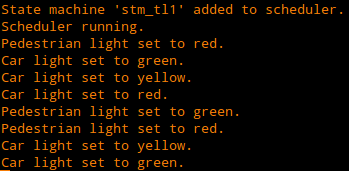
\includegraphics[scale=0.70]{traffic_light_output}
	\caption[Output of Traffic Light Controller test run (desktop)]{Console output resulting from the test run of the Traffic Light Controller state machine application.}
	\label{fig:traffic_light_output}
\end{figure}

\subsection{Two Communicating Applications}
\label{sec:client_server_app}
Our next step is to test the runtime system with more than a single state machine, so the scheduler has to do some actual scheduling. To achieve this, I designed some simple state machines working together to form a client and a server. To communicate between the client and the server, I designed state machines using \gls{tcp} sockets from the LuaSocket library.\footnote{\url{http://w3.impa.br/~diego/software/luasocket/}} The client application consists of one state machine for periodically generating requests (Fig.~\ref{fig:stm_event_gen}), one for displaying replies from the server (Fig.~\ref{fig:stm_print_message}) and one for sending and receiving messages over \gls{tcp} (Fig.~\ref{fig:stm_client_conn}). The server application consists of one state machine for handling requests (Fig.~\ref{fig:stm_request_handler}) and one for sending and receiving messages over \gls{tcp} (Fig.~\ref{fig:stm_server_conn}). The two \gls{tcp} state machines are almost identical, with the exception that the server side is by default in receive mode, while the client side is in send mode.
The Lua implementation for the request generating state machine is displayed in Code snip.~\ref{code:event_gen}, and the remaining implementations are publicly available on GitHub.\footnote{\url{https://github.com/Desarc/state_machine_rts/tree/master/client-server}}

\noindent
In addition to implementing the new state machines, I had to extend the runtime system with a simple \emph{message} format, enabling easy serialization and deserialization of object data to be sent over the network.

\noindent
Comparing the implementation of the request generator to the implementation of the Traffic Light Controller in Sect.~\ref{sec:impl_traffic_light}, we see that a lot of the code may be reused. We basically only need to change state and event definitions, implement any operations performed in transitions, and finally change the action-oriented list of transitions to reflect those of the current state machine. It requires only minimal work, and is not particularly error-prone because the code is simple and readable. This also applies to the other state machines implemented for this application, and implies that creating more complex applications, given the state machine template and a working runtime system, should be rather trivial.

\noindent
Running the two applications also produced the expected results: the client application periodically sends requests, these are handled by the server application, and the client application finally receives a response. The output produced is displayed in Fig.~\ref{fig:client_output} and~\ref{fig:server_output}.

\begin{figure}[htp]
	\centering
	\begin{minipage}{0.45\linewidth}
		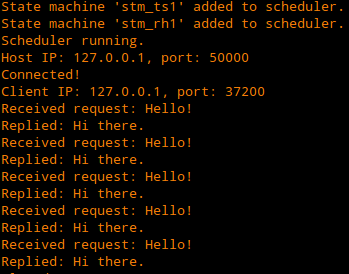
\includegraphics[scale=0.40]{server_output}
		\caption{Server-side console output from running the client-server application.}
		\label{fig:client_output}
	\end{minipage}
	\quad
	\begin{minipage}{0.45\linewidth}
		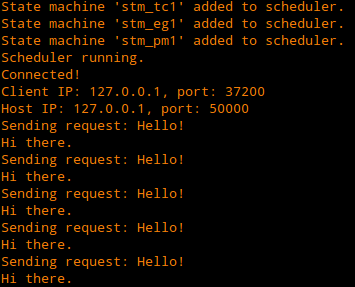
\includegraphics[scale=0.40]{client_output}
		\caption{Client-side console output from running the client-server application.}
		\label{fig:server_output}
	\end{minipage}
\end{figure}

\FloatBarrier
\section{Running the State Machine Applications in an Embedded Environment}
\label{sec:running_on_micro}
Now that we have a working runtime system with a few example state machine -based applications, the next step is to see how this system performs in an embedded environment. In Sect.~\ref{sec:lua_in_embedded}, I looked into some previous efforts towards running the Lua interpreter in an embedded environment. Since porting Lua to an embedded environment is beyond the scope of this project, I chose to use \emph{eLua} with the supported Stellaris LM3S9D92 microcontroller as the platform for these experiments.

\subsection{The LM3S9D92 Microcontroller}
\label{sec:microcontroller}
The Stellaris LM3S9D92 is a microcontroller produced by Texas Instruments.\footnote{\url{http://www.ti.com/product/lm3s9d92}} It is considered outdated and \emph{``not recommended for new designs''}, but since the purpose of these experiments is to look into how our software performs in a resource-constrained environment, this is not a problem. The microcontroller is considered a \emph{``high performance microcontroller with large memory''}~\cite{website:stellaris_micro}, roughly on par with microcontrollers like for example the Arduino Due.\footnote{\url{http://arduino.cc/en/Main/arduinoBoardDue}} It has the following primary specifications:

\begin{itemize}
	\item 32-bit ARM Cortex-M3 processor
	\item 96KB \gls{sdram}
	\item 512KB flash memory
\end{itemize}

\noindent
Additionally, the evaluation kit used supports the following \gls{io} peripherals:

\begin{itemize}
	\item Ethernet 10/100 port with two \gls{led} indicators
	\item User pushbutton and \gls{led}
	\item \gls{usb} 2.0 Full-Speed \gls{otg} port
	\item Oversized board pads for \gls{gpio} access
\end{itemize}

\noindent
Ethernet and \gls{tcp}/\gls{ip} is also supported by eLua for this platform, which should simplify the use of this feature in our state machines. Drivers interfacing with eLua for other peripherals do not seem to be present, but given eLua's open source, it should be possible to add these if needed.

\subsection{Running eLua on the Evaluation Kit Board}
\label{sec:running_elua}
In order to illustrate how quickly I was able to get the Lua interpreter up and running on the LM3S9D92, I have included a short description of the process in this section.

\noindent
The first step was to get the interface to the evaluation kit board up and running. The board has an FTDI chip\footnote{\url{http://www.ftdichip.com/FTProducts.htm}} converting between \gls{usb} and \gls{uart} interfaces, so in order to communicate with the board we only need to connect it via \gls{usb}. Texas Instruments also provide convenient desktop tools for connecting and flashing programs to the board, provided you are running on Windows. I simply had to install all the proper tools and drivers from the included CD, and turn the board on.

\noindent
The next step was to get eLua running on the microcontroller. Using the flashing tool provided with the kit, I simply downloaded the appropriate binary image from the eLua website and copied it over.

\noindent
The only challenge in this process was to find a suitable terminal emulator for Windows. The eLua wiki offered a few alternatives,\footnote{\url{http://wiki.eluaproject.net/Terminal\%20Emulators\%20for\%20eLua}} but many were outdated or didn't work properly. After trying out a few, I managed to connect using TeraTerm, and was able to run Lua scripts live through the eLua interpreter. Given the relative ease of this process, running Lua-based state machine applications seemed to be a very feasible option.

\subsection{Running the Initial State Machine Applications}
\label{sec:running_initial}
With Lua up and running on the evaluation kit board, the next step was to see if the runtime system with different state machine applications would run on it. In order to work on the embedded platform, some minor changes had to be done to the runtime system, particularly those that referenced \gls{os} functions. I had to replace the \emph{os.time()} function with the eLua equivalent \emph{tmr.read(tmr.SYS\_TIMER)} in the timer and scheduler objects. Also, because the eLua timers measure time in microseconds, I initially had to change all defined time constants. However, to make the difference between desktop and embedded versions of the runtime system a little smoother, I introduced a \emph{Timer.BASE} value representing the number of milliseconds in the timer object's base value for time measurement. This way we don't have to change timer constants in implemented state machines when changing from running in a desktop environment to running in an embedded environment. Similar changes were made to the scheduler, letting us choose which \emph{time} function to use depending on the current platform.

\subsubsection{The Traffic Light Controller Application}
After making the necessary changes to the code\footnote{\url{https://github.com/Desarc/state_machine_rts/tree/master/trafficlight-micro}} as described above, I copied it to the microcontroller's \gls{rom} and attempted to run the application. I was delighted to see that the application ran just as well on the microcontroller as it did in a desktop environment, producing similar output in a timely fashion. The results are displayed in Fig.~\ref{fig:traffic_light_output_micro}.

\begin{figure}[htp]
	\centering
	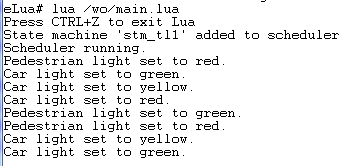
\includegraphics[scale=0.90]{traffic_light_output_micro}
	\caption[Output of Traffic Light Controller test run (microcontroller)]{Console output resulting from the test run of the Traffic Light Controller state machine application on the evaluation kit board.}
	\label{fig:traffic_light_output_micro}
\end{figure}

\subsubsection{The Client - Server Application}
When testing the client-server application on the evaluation kit board, I chose to make the microcontroller the active client, and let the desktop be the passive server. To make it run on the board, I had to make some additional changes to the code.\footnote{\url{https://github.com/Desarc/state_machine_rts/tree/master/client-server-micro}} The LuaSocket library is not available in eLua, but it has its own module for \gls{tcp}/\gls{ip} management, \emph{net}. To use this module instead, I only had to change the functions for connecting, sending and receiving on the network in the client state machine. All state, event and transition definitions fortunately remained the same.

\noindent
Running the application on the board produced almost identical results as in the desktop environment, with one exception: after about 14 requests, the client application running on the board runs out of memory, as displayed in Fig.~\ref{fig:client_output_micro}. This is where the trouble starts.

\begin{figure}[htp]
	\centering
	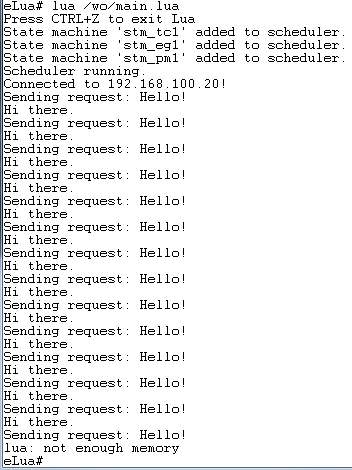
\includegraphics[scale=0.80]{client_output_micro}
	\caption[Output of client-server test run (microcontroller)]{Console output resulting from the test run of the client state machine application on the evaluation kit board.}
	\label{fig:client_output_micro}
\end{figure}

\noindent
Since running out of memory after a few seconds is not an option, some changes to the system must be made. These changes will be discussed in the following sections.

\section{Memory Use in the Runtime System}
\label{sec:memory_use}
Since the microcontroller quickly runs out of memory when running something as simple as the client-server application, some optimizations regarding memory use must be made. Since we are working in a resource-constrained environment, the worst case is that an application like this simply will use too much memory, and sufficient optimization is not possible. However, I initially made no considerations towards memory use when writing the code for the runtime system, so there is likely a lot of room for improvement.

\subsection{Analysis of Memory Use}
\label{sec:memory_analysis}
Fortunately, chapter 2 of \emph{Lua Programming Gems}~\cite{chapter:lua_performance_tips} offers some insight into which parts of our program could be using more memory than it really needs. Lua has some particularities in certain areas, especially when it comes to handling of tables and strings. A few interesting points mentioned in the book that are also relevant to the program in question, are listed below:

\paragraph{Closures} Variables and functions inside closures are created anew each time the closure is referenced. This means that the current scheme of encapsulating data inside closures creates new instances not only for the data contained, but for all the setters/getters and other functions declared in the same scope. This is likely to use a lot of extra memory, especially considering timer and event objects that may be instantiated very frequently.

\paragraph{Tables} Tables have various subtleties that may cause them to use more memory than necessary, especially if a large number of small tables is used. Additionally, freeing elements in a table will generally not reduce its size. The recommended approach is to attempt reuse of tables whenever possible, especially when tables are created inside loops. This could be an issue in the case where we continuously create new event and timer objects, and the garbage collector is too slow to reclaim those no longer in use.

\paragraph{Coroutines} Frequently creating and freeing coroutines creates some overhead, however this is mainly performance-related, and the garbage collector should generally clean up the extra memory used in good time. In our runtime system, this is unlikely to be an issue, as we only create one coroutine for each state machine instance, which stays with it for its complete lifetime.

\paragraph{Strings} Lua keeps a single copy of any string in memory, and thus all string variables contain only references to this value. While this will generally conserve memory and speed up many operations, there are some pitfalls. A simple example is a for-loop that builds a string from some values, one step at a time. Using regular string concatenation will create a copy in memory of all the intermediate strings as well as the final result, which is extremely inefficient. This could be a problem in our message object's \emph{serialize}, which does exactly that. However, the messages serialized are generally very short, and thus should not increase memory use dramatically.

\paragraph{The Garbage Collector} 
The garbage collector used by Lua is not meant for heavy tasks, and may struggle if there is a lot of garbage to collect. The best way to avoid this is to follow the principles of ``reuse and reduce'' as discussed in the paragraphs above, but it is also possible to change some parameters of the garbage collector to make it perform better in certain cases, or even control it manually.

\subsection{First Optimization of Memory Use}
\label{sec:first_optimalization}
Taking into account the various possible culprits of excessive memory use discussed in Sect.~\ref{sec:memory_analysis}, I decided that the encapsulation scheme with closure was likely to be the major problem. In addition to the smaller objects such as timers and events being instantiated frequently, the larger objects such as the scheduler and state machine implementations are duplicated within each local scope. This means that we most likely have to significantly reduce encapsulation, or possibly remove it completely.

\subsubsection{Code Changes}
Weighing the ``safety'' of encapsulation against the increased memory use, I decided it would probably be best to remove it completely, which is likely to make the runtime system safer with respect to running out of memory. The primary changes required are listed below, and the interested reader may find the complete code on GitHub.\footnote{\url{https://github.com/Desarc/state_machine_rts/tree/master/client-server-noencap}}

\begin{itemize}
	\item Instead of loading modules locally in each chunk, we can probably save some memory by making the \emph{main} chunk responsible for loading all required modules and making them globally available. This however likely to decrease performance significantly~\cite{chapter:lua_performance_tips}.
	\item Instead of declaring all member functions inside the \emph{new} closure, make the data ``publicly'' available, and reference member functions by use of inheritance. This is also likely to decrease performance, as member functions are now accessed through the \emph{\_\_index} metamethod.
\end{itemize}

\subsubsection{Result of Code Changes}
Removing encapsulation from the runtime system unfortunately required a significant amount of manual code changes to the implemented state machines, because virtually all references to object data or functions had to be changed. However, the change was worthwhile: when running the updated code on the microcontroller, there were no indications of memory problems, and the application seemed able to run indefinitely. It should be kept in mind that while we have reduced overall memory use, it's hard to tell if it increases over time, but hopefully the garbage collector is now able to deal with this properly.

\section{Measurements of Memory Overhead}
\label{sec:memory_overhead_measure}
In light of the memory troubles encountered in Sect.~\ref{sec:running_on_micro}, an important question to ask is how much extra memory a state machine application is using compared to an application performing the same task without the added overhead of the runtime system. If the memory overhead is significant, and further results in the possibility that we actually don't have enough, the use of a state machine -based system in the given context would be discouraged. The worst case would be that the garbage collector is not able to deal with the memory used by the runtime system, making it increase steadily.

\subsection{The Test Program}
\label{sec:test_program}
Measuring memory used by Lua is fortunately simple: the garbage collector provides a function, \emph{collectgarbage("count")} that returns the amount of memory currently used by Lua in KB. In order to test memory use for the runtime system, we simply design a state machine that periodically reads the current memory used, and logs this data somewhere. Since logging options are rather limited on the microcontroller, a better option is to aggregate the data over a period and send it over \gls{tcp}/\gls{ip} to a desktop application which handles the actual logging. In addition to measuring memory, we also want to simulate the microcontroller performing some useful task simultaneously, to make it more realistic. The chosen task, displayed in Code snip.~\ref{code:simple_task} is perhaps itself not very realistic in this context, but it serves the purpose of consuming some \gls{cpu} time and memory. This task is simply implemented in its own state machine, running in parallel with the memory measurements.

\begin{listing}[htp]
\begin{luacode}
local task_size = 500

local function simple_task()
	for i=1,task_size do
		q = i*i
	end
end
\end{luacode}
	\caption{Code for simple task used in memory overhead testing.}
	\label{code:simple_task}
\end{listing}

\noindent
For comparison, we create a simple program performing roughly the same tasks as the state machine application: continuously running the simple task, in addition to making periodic memory usage measurements and sending aggregate data to a desktop application. The code for the test program is included in Code snip.~\ref{code:memory_overhead_test}, and the full code used for this part is available on GitHub.\footnote{\url{https://github.com/Desarc/state_machine_rts/tree/master/mem-nonopt}}

\subsection{Results of the First Comparison}
\label{sec:first_comparison}
Figure~\ref{fig:memory_use_first} shows a graph representation of the memory used as a function of time. It is clear that the memory overhead of running this program as a state machine application is significant. The simple program uses only 14,7KB on average with a maximum of 17,3KB, while the state machine application uses 55,6KB of dynamic memory on average, with a maximum of over 66KB in this short period, almost 4 times as much. The huge difference in average memory used implies that the overhead of the runtime system could be as high as 40KB, close to half of the available dynamic memory, regardless of which state machine application is implemented.

\noindent
Additionally, the high maximum value is worth noticing. In order to check the actual available dynamic memory, I reran the encapsulated version of the runtime system from Sect.~\ref{sec:impl_runtime_support} with the state machines for measuring and logging memory use.\footnote{\url{https://github.com/Desarc/state_machine_rts/tree/master/mem-encap}} Unsurprisingly the program did not run for very long before running out of memory, but the interesting part was that the memory readings it managed to log before stopping, indicated that the program ran out of memory at around 68KB. The last received reading was 63,8KB, but we should assume that memory use at the time of the ``crash'' was higher, and judging by the previous readings, an increase of 3-4KB in the short time period seems likely. This implies that the actual maximum limit for memory use is somewhere around 68KB (indicated by the magenta-colored line in Fig.~\ref{fig:memory_use_first}), meaning that a measured value of 66KB is a little too close to this limit for ``comfort''. The reason for this limit being around 68KB, which is quite far from the microcontroller capability of 96KB \gls{ram}, is likely that some of the memory is used for controlling \gls{io} peripherals that are not directly part of the eLua \gls{vm}, such as the \gls{usb} interface.

\begin{figure}[htp]
	\centering
	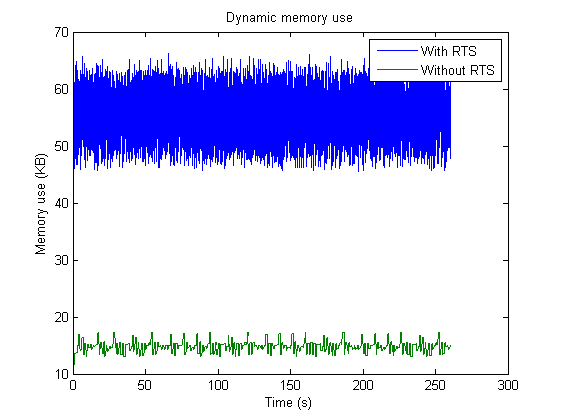
\includegraphics[scale=0.85]{memory_use_first}
	\caption[Results of first memory overhead test]{Compared memory use of the test program running as a state machine application within the runtime system, and as a simple standalone program.}
	\label{fig:memory_use_first}
\end{figure}

\noindent
In order to justify the use of Lua state machine applications in embedded environments, we need to find out if it is possible to further reduce the memory overhead produced by the runtime system.

\subsection{Further Optimizations of Memory Use}
\label{sec:more_optimization}
Given the huge memory overhead observed during the testing in Sect.~\ref{sec:first_comparison}, we most likely have to make some drastic changes to the code of our runtime system. In Sect.~\ref{sec:memory_analysis}, various potential issues increasing dynamic memory use are discussed. The issue of closures has already been addressed, so the next step to explore the other options.

\paragraph{Reuse} During the lifetime of a state machine application, it is likely that a large number of timer and event objects will be created. As soon as the event or timer is consumed, it will likely be reclaimed by the garbage collector, but depending on the garbage collector's speed, this may not happen right away. Thus, we risk seeing temporary spikes in dynamic memory use, most likely similar to the spikes observed in Fig.~\ref{fig:memory_use_first}. As an alternative to this scheme, we can reduce the work that needs to be done by the garbage collector by reducing event and timer objects when creating new timers and events. The risk of seeing spikes is then probably reduced, however this is not likely to affect average memory use much. As a bonus, reusing events and timers is probably a little faster than instantiating new objects every time. It should be noted that the optimization gains from this approach depends on the state machine application being run. State machines that frequently consume one event and generates another save more than state machines that consume one event to generate many, which in turn may or may not generate new events.

\paragraph{Strings} Another possible memory sink is the string concatenations performed by the message objects, as well as the state machine measuring memory use. These should however be the same for both test programs, since they send the same messages with an equal amount of data, but it is still worth looking into. Even if the relative difference in memory use may not be affected, we can still reduce average memory use for the runtime system. Depending on how fast these strings are reclaimed by the garbage collector, this reduction may be significant. The recommended approach is to use a table containing only the string values to be concatenated, and then use the \emph{table.concat} function. This should also give a significant performance increase for these tasks~\cite{chapter:lua_performance_tips}.

\paragraph{Coroutines} Since coroutines in Lua have their own stack, it is likely that events and timers passed between state machines and the scheduler will be created locally within each coroutine, and thus duplicated. In addition to temporarily using extra memory, this will reduce the effect we get from reusing event and timer objects. Also, using coroutines in itself likely creates some additional overhead, but this should not be significant.

\paragraph{Garbage Collection} Tuning the garbage collector to be more aggressive is another way to reduce memory use, however this also happens at the cost of performance. However, looking at the results in Fig.~\ref{fig:memory_use_first}, the frequent maxima and minima as well as the large relative difference between them, imply that the garbage collector is already being quite aggressive. This also makes sense, considering the amount of new memory that is frequently allocated when new event and timer objects are created.

\noindent
eLua additionally offers another alternative for handling garbage collection in situations where the remaining available memory is low, namely the \gls{egc}. This tool allows Lua to run garbage collection in some situations where this is normally not possible, for example when we reach a certain memory limit~\cite{website:elua_egc}. While this can be useful for avoiding running out of memory when we're already close to the limit, it doesn't really solve our problem, and is best used for safety measures.

\paragraph{LTR} The people working on eLua recognize the need for memory-effective software in resource constrained environments, and have developed \gls{ltr} to improve the situation for eLua. \emph{``\gls{ltr} is a Lua patch that significantly decreases the \gls{ram} usage of Lua scripts, thus making it possible to run large Lua programs on systems with limited \gls{ram}''}~\cite{website:elua_ltr}. The website advertises that enabling the patch should reduce the eLua memory overhead from around 27KB to only 5.42KB on the LM3S platform, however at the cost of performance. Unfortunately, a quick test showed that the \gls{ltr} patch was already enabled for my build of eLua. While having this patch enabled when we're struggling with memory use is obviously a good thing, it also implies that without this specific patch for eLua, making our runtime system fit into the \gls{ram} of the microcontroller would have been much more difficult.

\subsection{Measurements on the Optimized Runtime System}
\label{sec:opt_rts}
Considering the possibilities for further optimization discussed in Sect.~\ref{sec:more_optimization}, I decided to try a few different options, and see how they affected memory use. First, I changed all handling of string concatenation to the recommended approach with \emph{table.concat}. Next, I made state machines attempt reuse of event and timer objects whenever possible, creating new ones only when they had to. The full code for this optimized system is available on GitHub.\footnote{\url{https://github.com/Desarc/state_machine_rts/tree/master/mem-opt}} With some luck, these changes would significantly reduce and and stabilize memory use. Additionally, I created a version of the runtime system without coroutines\footnote{\url{https://github.com/Desarc/state_machine_rts/tree/master/no-coroutine}} as the way of handing execution control to a state machine, to see how much of an impact this would have on memory use.

\noindent
The results of running these optimized programs are displayed in Fig.~\ref{fig:memory_use_second}, and fortunately show some improvements. Some observations are listed below:

\begin{itemize}
	\item For the optimized system, average memory use has been reduced from 55,6KB to 48,3KB, and the maximum from 66KB to 55,7KB. This is an improvement of roughly 13\%, and puts us at a more comfortable distance from the maximum limit (indicated by the magenta line).
	\item The optimized system without coroutines is slightly sparser, with an average memory use of 44,3KB.
	\item With the same optimizations applied, the comparison program actually performs slightly worse on average, but the difference is very small.
	\item Since fewer new objects are created (and fewer old ones are becoming obsolete), the garbage collector activity is significantly decreased, to the point where we can clearly see the garbage collection cycles. This likely gives a performance boost to our system, since normal execution will be interrupted less.
	\item Average memory use is still more than 3 times higher for the state machine application.
\end{itemize}

\begin{figure}[htp]
	\centering
	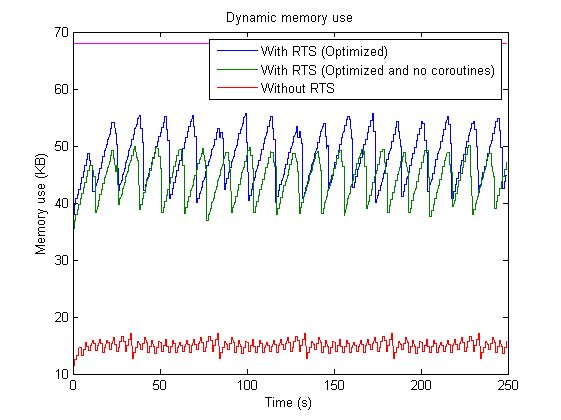
\includegraphics[scale=0.85]{memory_use_second}
	\caption[Results of second memory overhead test]{Compared memory use of the test program running as a state machine application within the optimized runtime system.}
	\label{fig:memory_use_second}
\end{figure}

\noindent
While we see a definite improvement over the initial system, the memory overhead is still quite high, and may potentially severely limit the types of applications we are able to develop. On the bright side, the decreased activity of the garbage collector gives us more room for tinkering with its parameters, with the potential of reducing average and peak memory use. The next section will explore these options further.

\subsection{Tinkering With the Garbage Collector}
\label{sec:gc_tinkering}
The capabilities of the garbage collector in Lua are briefly discussed in Sect.~\ref{sec:memory_analysis} and ~\ref{sec:more_optimization}. Given the results observed in Sect.~\ref{sec:opt_rts}, it seems likely that by changing some of the garbage collectors parameters, we can make it more aggressive and hopefully reduce average memory use. In addition to the possibility for manual control (collect, stop, restart), the Lua garbage collector has two controllable parameters: step multiplier and pause~\cite[ch. 2.10]{manual:lua_reference_manual}.

\paragraph{Pause} The pause parameter decides how long the garbage collector should wait before starting a new collection cycle. Decreasing the parameter makes the garbage collector less aggressive, while increasing makes it more. The default value is 200, and values smaller than 100 means there is no pause. A quick check of this value in the context of eLua shows that it is already set to 110, which should make the garbage collector quite aggressive. It is therefore unlikely that we have much to gain from further decreasing its value.

\paragraph{Step Multiplier} The step multiplier parameter roughly decides how much work the garbage collector does with each incremental step. This means that increasing its value makes the garbage collector more aggressive, and like the pause parameter its default value is 200. A quick check shows that this is also the default value used by eLua, meaning there could be potential for some gain by increasing it.

\paragraph{Manual Control} While manual control has the potential to reduce memory use at the times when it's really needed, this probably requires knowledge of the specific application running within the runtime system, making it hard to know exactly when these times are. An option could be to experiment with the \gls{egc} mentioned in Sect.~\ref{sec:more_optimization}, but the results are hard to predict. Worst case, it actually provides us with more problems, such as getting stuck in an eternal loop of garbage collection.

\noindent
Running the optimized (with coroutines) memory-measurement application with different values for the step multiplier provides the results displayed in Fig.~\ref{fig:memory_use_opt}. Increasing the step multiplier from 200 to 600 decreases average memory use from 48,3KB to 42,5KB and peak memory use from 56KB to 45KB. Further increases of the step multiplier have a significantly smaller effect on the memory use, and we should keep in mind that performance decreases when the garbage collector has to do more work. Overall, dynamic memory use is a lot more stable, and we are getting a little closer to an acceptable amount of overhead. However, at this point I've run out of ideas on how to improve the runtime system further, so we have to accept a memory overhead of roughly 27KB for now.

\begin{figure}[htp]
	\centering
	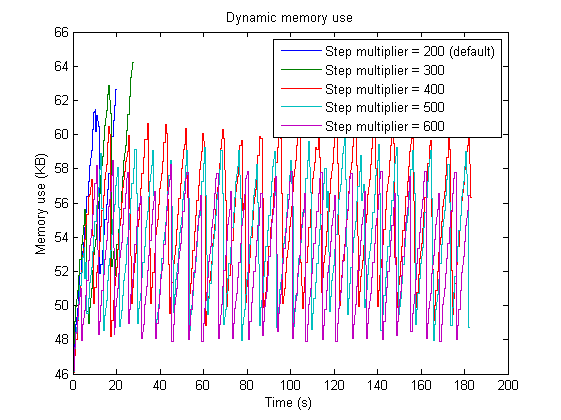
\includegraphics[scale=0.85]{memory_use_opt}
	\caption[Results of tinkering with the garbage collector for the state machine application]{Compared memory use of the state machine system for different values of the garbage collector's step multiplier parameter.}
	\label{fig:memory_use_opt}
\end{figure}

\subsection{Some Additional Notes on Memory Overhead}
\label{sec:mem_overhead_notes}
While the previous sections offer some insights into potential memory problems we may encounter with a Lua-based state machine system in an embedded environment, we should keep in mind that the tests and measurements performed are quite specific, and over a relatively short period of time. Results may vary depending on the actual application that is run within the context of the runtime system, and for a large number of applications, the added memory overhead is not likely to be a problem given that the memory use is fairly stable.

\noindent
However, the most important point to consider is probably that the runtime system used for these measurements is just the bare minimum that is required for functional use. With a more complete, production-quality system, we would probably like to add quite a few extra features to the runtime system, which may increase overhead with respect to both dynamic memory use and performance. We already experienced that a single concept such as encapsulation of object data increased memory use so dramatically that we would quickly run out, which implies that some of the additional features we might like in a production-quality system may not be achievable in this context.

\noindent
The specific application should also be considered when comparing to the test program running without a runtime system. In the tests performed in the previous sections, our application is very simple, meaning the relative memory overhead becomes quite big. In Sect.~\ref{sec:opt_rts}, we saw that the same optimizations applied to the test program did not improve memory usage, however there is likely to be more room for such optimizations in a more complex program. On the other hand, complex programs are generally more difficult to optimize, which speaks in favor of the state machine -based system. When developing with state machines, most of the optimization will be done in the runtime system, making things simpler for the application developer.

\noindent
There are some additional ways to reduce the memory overhead of our runtime system, but they require more advanced adaptations. The eLua FAQ suggests that we can precompile our Lua code to bytecode and build it directly into the \gls{rom} file system of eLua~\cite{website:elua_faq}. This is likely to provide significant results, since we may then put all our prototypes in \gls{rom}. However, if application developers want to put the prototypes for their state machines in \gls{rom}, this approach requires them to be able to build eLua, which may require a lot of extra work. Another option is to implement the memory-heavy parts of the runtime system in C. This is a likely solution for a production-quality system, but goes beyond the scope of this project.

\FloatBarrier
\section{Performance Overhead of the Runtime System}
\label{sec:performance_overhead}
So far in our experiments, we have only considered how well our runtime system performs with respect to memory use. A lot of the steps that were taken to reduce memory overhead in Sect.~\ref{sec:memory_use} and~\ref{sec:memory_overhead_measure} are likely to decrease performance in our application, and it is probably a good idea to find out roughly how much. Additionally, like with memory, a speed comparison with a non state machine application to measure the performance overhead is appropriate. The following sections describe the results from these tests.

\subsection{The Test Code}
\label{sec:performance_test_code}
There are many ways of measuring performance in software. A typical way is to run benchmarks with a set algorithms, but this is more suited for testing language implementations or hardware. Another approach is performance profiling, which may be done in Lua by use of the \emph{debug} and \emph{os} libraries, however since the \emph{os} library is not available on the microcontroller, this may prove difficult to achieve. Instead, we may use a simpler scheme: create a real or fictional task, such as the one used for memory overhead testing, and see how the runtime system performs compared to a non state machine program when running this task several times in succession. Additionally, we may do this for variable task sizes, to see how big the impact of the performance overhead is relative to how long it takes to perform the task. Using the simple task described in Code snip.~\ref{code:simple_task}, we design a state machine that continuously runs this task while measuring the time it takes between completions. The full code used for this test is available on GitHub.\footnote{\url{https://github.com/Desarc/state_machine_rts/tree/master/calc-overhead-opt}}

\subsection{Measuring Performance Overhead of the Runtime System}
\label{sec:performance_overhead_measure}
Running the test code described in the previous section, we use values for task\_size ranging from 10 to 50000, and values for task\_repeats ranging from 1 to 500. Additionally, results are calculated by averaging the measurements from 10 runs for each set of parameters. Table~\ref{tab:task_size_time} gives an overview of how long it takes to run a task on the microcontroller, given the task\_size parameter. We see that the time required to complete a task is almost directly proportional to the value of task\_size, and that multiplying the value of task\_size by 10 gives a fairly close approximation to the time it takes to run the task in microseconds.

\begin{table}
	\centering
	\begin{tabulary}{\textwidth}{| C | C | C |}
		\hline
		task\_size & Time ($\mu$s) & Adjusted time ($\mu$s) \\
		\hline
		10 & 235 & 111 \\
		\hline
		50 & 623 & 498 \\
		\hline
		100 & 1108 & 983 \\
		\hline
		500 & 4963 & 4838 \\
		\hline
		1000 & 9781 & 9657 \\
		\hline
		5000 & 48363 & 48238 \\
		\hline
		10000 & 96578 & 96453 \\
		\hline
		50000 & 482358 & 482233 \\
		\hline
	\end{tabulary}
	\caption[Values for task\_size and their respective execution times]{Values for task\_size and their respective execution times. The adjusted time represents the actual time the task takes, when we subtract the time it takes to read timer values, approximately 125 $\mu$s.}
	\label{tab:task_size_time}
\end{table}

\noindent
Comparing the results from running the state machine test application and the test program, we get the results displayed in Fig.~\ref{fig:performance_overhead_rel}. We see that for smallest tasks tested, the state machine application takes more than 5 times as long as the simple test program to complete the task. As the size of the task increases, this difference becomes less significant, and at 100ms it is hardly noticeable. Considering that the state machine application has some overhead associated with each run of the task, this is expected, but we should analyze the data a little further to get an impression of the impact this has on any potential real application.

\begin{figure}[htp]
	\centering
	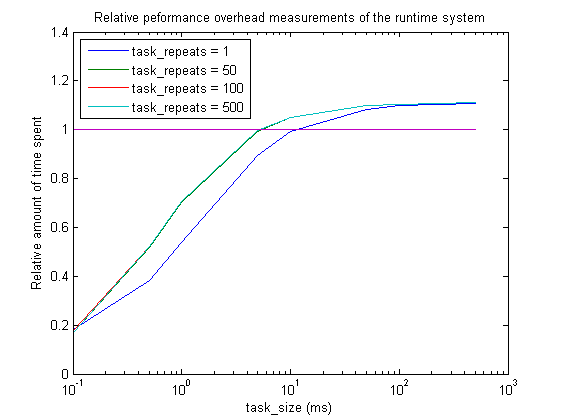
\includegraphics[scale=0.85]{performance_overhead_rel}
	\caption[Results of performance overhead test, relative comparison]{Relative comparison of time spent running the simple task, where the value on the y-axis represents the time spent by the test program divided by the time spent by the state machine application.}
	\label{fig:performance_overhead_rel}
\end{figure}

\noindent
Adjusting the results for number of repeats and task size, we get the relative amount of overhead compared to the amount of useful work done. Figure~\ref{fig:performance_overhead_abs} shows the results of these computations. We see that for the special case where we only perform the given task once, the processing overhead is significant for small tasks, with up to 5/6 of the processing time being spent on runtime system overhead. However, it is more realistic to look at the cases where a task is repeated over time. As long as the task is repeated more than a few times, the exact number does not seem to make a real difference (the curve for \emph{task\_size = 50} almost completely fits the curve for \emph{task\_size = 100} in Fig.~\ref{fig:performance_overhead_abs}). While the processing overhead is still quite high for small tasks (up to almost 3/4) when the task is repeated over time, it is much smaller than when running a task once, which implies that there is some ``initial setup'' computation performed in the runtime system. For tasks taking around 10ms or more to complete, this processing overhead becomes insignificant.

\noindent
In addition to showing processing overhead, the results in Fig.~\ref{fig:performance_overhead_abs} give us an indication of how frequently the system is able to handle tasks of various sizes before these tasks start to become delayed in time. The system will for example not be able to handle scheduling tasks that take 100$\mu$s with a frequency of 1/5000, because even though there is plenty of time to complete 5000 tasks taking 100$\mu$s in one second, we also have to account for the runtime system overhead, which in this case is more than 250$\mu$s per 100$\mu$s of useful work. This means that a state machine task taking 100$\mu$s will in reality use around 350$\mu$s of processing time, meaning it can be scheduled at most with a frequency of roughly 1/2850 to avoid experiencing delay. Similar considerations must be made when considering bigger tasks, at least up to 10ms.

\begin{figure}[htp]
	\centering
	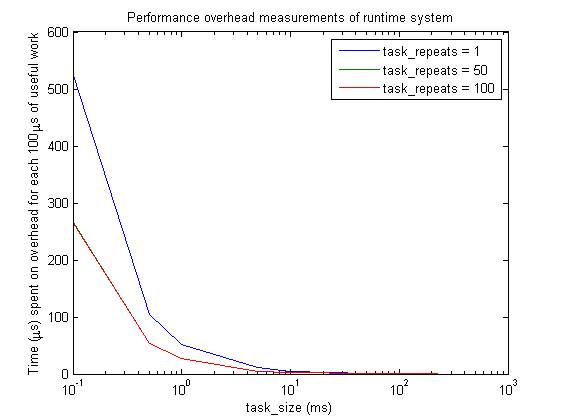
\includegraphics[scale=0.85]{performance_overhead_abs}
	\caption[Results of performance overhead test, absolute comparison]{Measurements of overhead time required when running the simple task, where the value on the y-axis represents the time spent on overhead by the runtime system for each 100$\mu$s of useful work.}
	\label{fig:performance_overhead_abs}
\end{figure}

\noindent
In order to get an impression of how the results in Fig.~\ref{fig:performance_overhead_abs} relate to real tasks a state machine application might perform, time required to send messages of various sizes over \gls{tcp}/\gls{ip} was measured. A simple test program\footnote{\url{https://github.com/Desarc/state_machine_rts/tree/master/ethernet-send}} was loaded onto the microcontroller, and the results from these measurements are displayed in Tab.~\ref{tab:ethernet_send_times}. Surprisingly, messages longer than 100 characters apparently take less time to send, however this is not that relevant. The important point is that sending a message over \gls{tcp}/\gls{ip} takes between 180ms and 200ms, which judging by the results in Fig.~\ref{fig:performance_overhead_abs} will not be affected significantly by the runtime system processing overhead. It seems that for many real tasks, the processing overhead of the runtime system may be negligible, but more tests should be run in order to arrive at a more definite conclusion.

\begin{table}
	\centering
	\begin{tabulary}{\textwidth}{| C | C |}
		\hline
		Message length (characters) & Time (ms) \\
		\hline
		10 & 179 \\
		\hline
		100 & 198 \\
		\hline
		200 & 196 \\
		\hline
		500 & 192 \\
		\hline
		1000 & 181 \\
		\hline
	\end{tabulary}
	\caption[Time required to send a message over TCP/IP in eLua]{Values for message size and the time it takes to send the message over \gls{tcp}/\gls{ip} using eLua's \emph{net} module.}
	\label{tab:ethernet_send_times}
\end{table}

\subsection{Comparing Performance to the First Version of the Runtime System}
\label{sec:comp_performance_overhead}
Compared to the runtime support system proposed in Sect.~\ref{sec:impl_runtime_support}, the memory-optimized version presented in Sect.~\ref{sec:opt_rts} has some significant differences. The various changes described in Sect.~\ref{sec:memory_analysis} and~\ref{sec:more_optimization} were expected to individually both increase and decrease performance, so it is hard to predict what the final result is. To find out, we run the same state machine program described in Sect~\ref{sec:performance_test_code} also with the first version of the runtime system,\footnote{\url{https://github.com/Desarc/state_machine_rts/tree/master/calc-overhead-nonopt}} and compare the results with those from Sect.~\ref{sec:performance_overhead_measure}. Since results seem to be very similar independent of the number of times we run the task, we use 100 as a fixed value for this parameter.

\noindent
The compared results are displayed in Fig.~\ref{fig:performance_overhead_comp}. We see that the first version of the runtime system actually performs a little worse than the memory optimized system, so by optimizing memory use, we have also inadvertently made the runtime system more efficient with respect to processing overhead. This clearly speaks in favor of the optimized version.

\begin{figure}[htp]
	\centering
	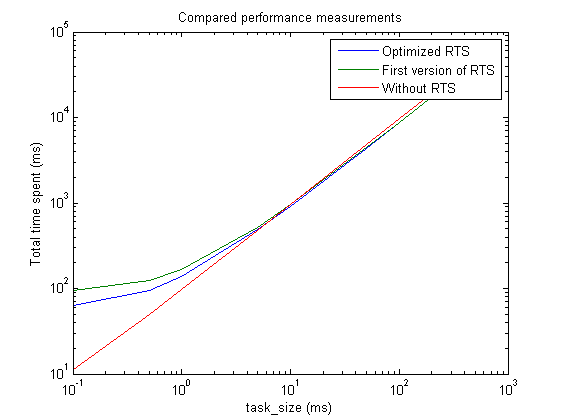
\includegraphics[scale=0.85]{performance_overhead_comp}
	\caption[Results of performance comparison with the first version of the runtime system]{Compared times required to run a task of the given size 100 times with the first \gls{rts}, the optimized \gls{rts} and without \gls{rts} support.}
	\label{fig:performance_overhead_comp}
\end{figure}

\FloatBarrier
\section{A More Complete State Machine Application}
\label{sec:complete_app}
As a final way of testing the runtime system, a more complete and realistic state machine should be implemented on the microcontroller, providing some additional insight into how the runtime system performs in an embedded environment. Ideally, this application would make use of sensors and the like to make some kind of measurements or observation, as well as listen to commands from a central server and regularly update it with data. There are many possible and vastly different applications one might think to implement in the given context, but this represents a likely use case. However, implementing this application within our Lua state machine runtime system is not as simple as it may seem. Some of the challenges encountered are discussed in the following paragraph.

\paragraph{Lack of Appropriate Peripherals} This is not directly related to the runtime system, but to the choice of microcontroller we use for testing. The EKK-LM3S9D92 evaluation kit unfortunately does not have any kind of sensors attached, so the only peripherals we may use in our application is a single \gls{led}, a single pushbutton and the Ethernet interface. This limits our options for developing a more complete example application.

\paragraph{Limited Peripheral Support in eLua} While working with the \gls{tcp}/\gls{ip} Ethernet interface on the LM3S platform is well supported by eLua, accessing the \gls{led} and pushbutton proved more difficult. eLua does not offer any separate modules for working with these peripherals, and digging through the limited \gls{gpio} documentation provided little insight as to if or how we may use the \gls{gpio} module for this purpose. Another option we have is to write our own driver module for the pushbutton and \gls{led} in C, and bind this module to Lua functions. Interfacing with C code is considered one of Lua's major strengths~\cite{inproceedings:the_evolution_of_lua}, so this should not be too difficult. However, in order to use the driver module, we will also most likely have to build it into the eLua image on the microcontroller, which leads to even more extra work. The purpose of our runtime system is after all to provide a simple interface for application development, and these advantages are quickly diminished when the developers have to dig into C code for peripheral support and building their own version the whole support system.

\paragraph{Support for Parallelism} Without support for real parallelism in Lua, it is challenging to create an application that serves both as an active ``client'' and a ``server''. If we want to continuously do useful work in our application, we are unable to listen for events and signals from external sources, as mentioned in Sect.~\ref{sec:runtime_system_issues}. One option is to periodically listen for external signals for a short time, but depending on how often and how long we listen, we risk missing a lot of the signals. Additionally, performing this task could in the worst case provide a relatively large amount of overhead, depending on how often external signals are actually received. In order to handle proper concurrency, we probably have to extend our runtime system with some kind of real parallelism, which may prove challenging in an embedded environment.

\noindent
It should be noted that while challenging, implementing support for asynchronous reception of external events is still feasible in this context, with some assumptions. As mentioned in Sect.~\ref{sec:runtime_system_issues}, if external event is buffered (for example at the sender's outgoing socket), we could let the runtime system periodically run a coroutine that checks this buffer. Given the results in Sect.~\ref{sec:performance_overhead_measure}, the extra overhead required for this routine may not be significant, depending on the tasks performed by the active state machines. With this approach, we delegate the responsibility for real parallelism to the ``client''-side of the application (it may have to receive data on one socket while at the same time having data buffered and ready for sending on another).

\paragraph{Summary} Simply put, there are some significant challenges that must be overcome in order to be able to develop more than simple applications within our runtime system. The choice of eLua as the underlying platform for the Lua interpreter has some impact on this, as it imposes some limitations on our Lua environment. But considering that eLua is still only in version 0.9, this might improve in the future. However, for a production-quality state machine runtime system, it might be safer to develop a separate and more specialized Lua platform for embedded systems.

%\chapter{Conclusion}

<Conclusion here>

%\chapter{Misc}

\section{Compiling Lua}
\label{sec:compiling}

http://lua-users.org/wiki/LuaCompilerInLua
http://luajit.org/luajit.html
http://www.lua.org/manual/5.1/luac.html


\section{Lua on embedded systems}

\subsection{Mihini}

http://www.eclipse.org/mihini/
http://wiki.eclipse.org/Mihini
http://blog.benjamin-cabe.com/2012/08/16/introducing-mihini
http://wiki.eclipse.org/Mihini/Run\_Mihini\_on\_an\_Open\_Hardware\_platform
http://andypiper.co.uk/tag/mihini/
http://beagleboard.org/
http://www.raspberrypi.org/
http://wiki.eclipse.org/Mihini/EclipseCon2013\_Tutorial

http://wiki.eclipse.org/images/1/16/M3DAPresentation.pdf

Run a simple C I/O program on Arduino, connect to RaspberryPi or BeagleBoard running Mihini with state machine and runtime system?

Koneki - remote execution

M3DA - binary serialization, security

\subsection{MQTT}
https://github.com/geekscape/mqtt\_lua
http://mqtt.org/
http://git.eclipse.org/c/paho/org.eclipse.paho.mqtt.lua.git/
http://www.eclipse.org/paho/


\subsection{Routers}
https://openwrt.org/

\subsection{Other}
Lua programming gems, ch. 26
%% include here the other chapters

\renewcommand*{\bibname}{References}
\bibliographystyle{alpha}
\bibliography{main}

%% Uncomment the following if you have any appendix
% \appendix
% \addtocontents{toc}{%
%  \protect\vspace{1em}% 
%  \protect\noindent \bfseries \appendixtocname\protect\par
%  \protect\vspace{-.5em}%
% }
% \renewcommand{\chaptername}{\appendixname}
%% include below possible appendices (chapters)


\end{document} 
